%
% $XORP: xorp/docs/pim/pim_arch.tex,v 1.5 2003/06/05 07:07:51 pavlin Exp $
%

\documentclass[11pt]{article}

%\usepackage[dvips]{changebar}

\usepackage{subfigure}
\usepackage{fullpage}
\usepackage{setspace}
\usepackage{times}
\usepackage{latexsym}
\usepackage{psfig}
\usepackage{graphicx}
\usepackage{xspace}
\usepackage{color}
\usepackage{amsmath}
%\usepackage[dvipdf]{graphics}
%\usepackage[dvips]{graphicx}
%\usepackage{xorp}

\definecolor{gray}{rgb}{0.5,0.5,0.5}
\newcommand{\etc}{\emph{etc.}\xspace}
\newcommand{\ie}{\emph{i.e.,}\xspace}
\newcommand{\eg}{\emph{e.g.,}\xspace}
%\newcommand{\comment}[1]{{\color{gray}[\textsf{#1}]}}
\newcommand{\comment}[1]{}

% Changebar stuff
% \newenvironment{colorcode}{\color{blue}}{}
% \renewcommand{\cbstart}{\begin{colorcode}}
% \renewcommand{\cbend}{\end{colorcode}}

% \pagestyle{empty}

\begin{document}

\title{XORP PIM-SM Routing Daemon \\
\vspace{1ex}
Version 0.3}
\author{ XORP Project					\\
	 International Computer Science Institute	\\
	 Berkeley, CA 94704, USA			\\
	 {\it feedback@xorp.org}
}
\date{June 9, 2003}

\maketitle

\thispagestyle{empty}


%%%%%%%%%%%%%%%%%%%%%%%%%%%%%%%%%%%%%%%%%%%%%%%%%%%%%%%%%%%%%%%%%%%%%%%
\section{Introduction}


%%%%%%%%%%%%%%%%%%%%%%%%%%%%%%%%%%%%%%%%%%%
\subsection{Overview}

This document provides an overview of the XORP PIM-SM~\cite{PIM-SM}
Routing Daemon. It is intended to provide a starting point for software
developers who wish to modify this software.

A router running PIM-SM interacts with other PIM-SM routers and
multicast group members, computes the multicast routing state, and installs
the corresponding multicast forwarding state in the multicast forwarding
engine.

The chosen architecture for the XORP PIM-SM implementation emphasizes on
correctness and extensibility rather than high performance or minimal
memory footprint. PIM-SM is a fairly complicated protocol, therefore it
is very important that the implementation follows closely the protocol
specification. Otherwise, premature optimization or ``cutting corners''
might introduce problems that are difficult to find. Only after the
implementation is well tested, we would
try to optimize those parts of the implementation that should prove
to be a bottleneck.

Currently (June 2003), the PIM-SM implementation is based
on the specification in the following documents:

\begin{itemize}
  \item \verb=draft-ietf-pim-sm-v2-new-05.{ps,txt}= (The core PIM-SM
  specification).
  \item \verb=draft-ietf-pim-sm-bsr-03.{ps,txt}= (The Bootstrap mechanism
  specification).
\end{itemize}

The only major features not implemented yet are SSM support and security.


%%%%%%%%%%%%%%%%%%%%%%%%%%%%%%%%%%%%%%%%%%%
\subsection{Acronyms}

Acronyms used in this document:

\begin{itemize}

  \item {\bf MFC}: {\bf M}ulticast {\bf F}orwarding {\bf C}ache: another
  name for an entry in the multicast forwarding engine (typically used
  on UNIX systems).

  \item {\bf MFEA}: {\bf M}ulticast {\bf F}orwarding {\bf E}ngine
  {\bf A}bstraction

  \item {\bf MLD/IGMP}: {\bf M}ulticast {\bf L}istener {\bf D}iscovery/{\bf
  I}nternet {\bf G}roup {\bf M}anagement {\bf P}rotocol

  \item {\bf MRIB}: {\bf M}ulticast {\bf R}outing {\bf I}nformation
  {\bf B}ase

  \item {\bf PIM-SM}: {\bf P}rotocol {\bf I}ndependent {\bf M}ulticast--{\bf
  S}parse {\bf M}ode

  \item {\bf RIB}: {\bf R}outing {\bf I}nformation {\bf B}ase

\end{itemize}


%%%%%%%%%%%%%%%%%%%%%%%%%%%%%%%%%%%%%%%%%%%
\subsection{PIM-SM Design Architecture Overview}

\begin{figure}[htbp]
  \begin{center}
    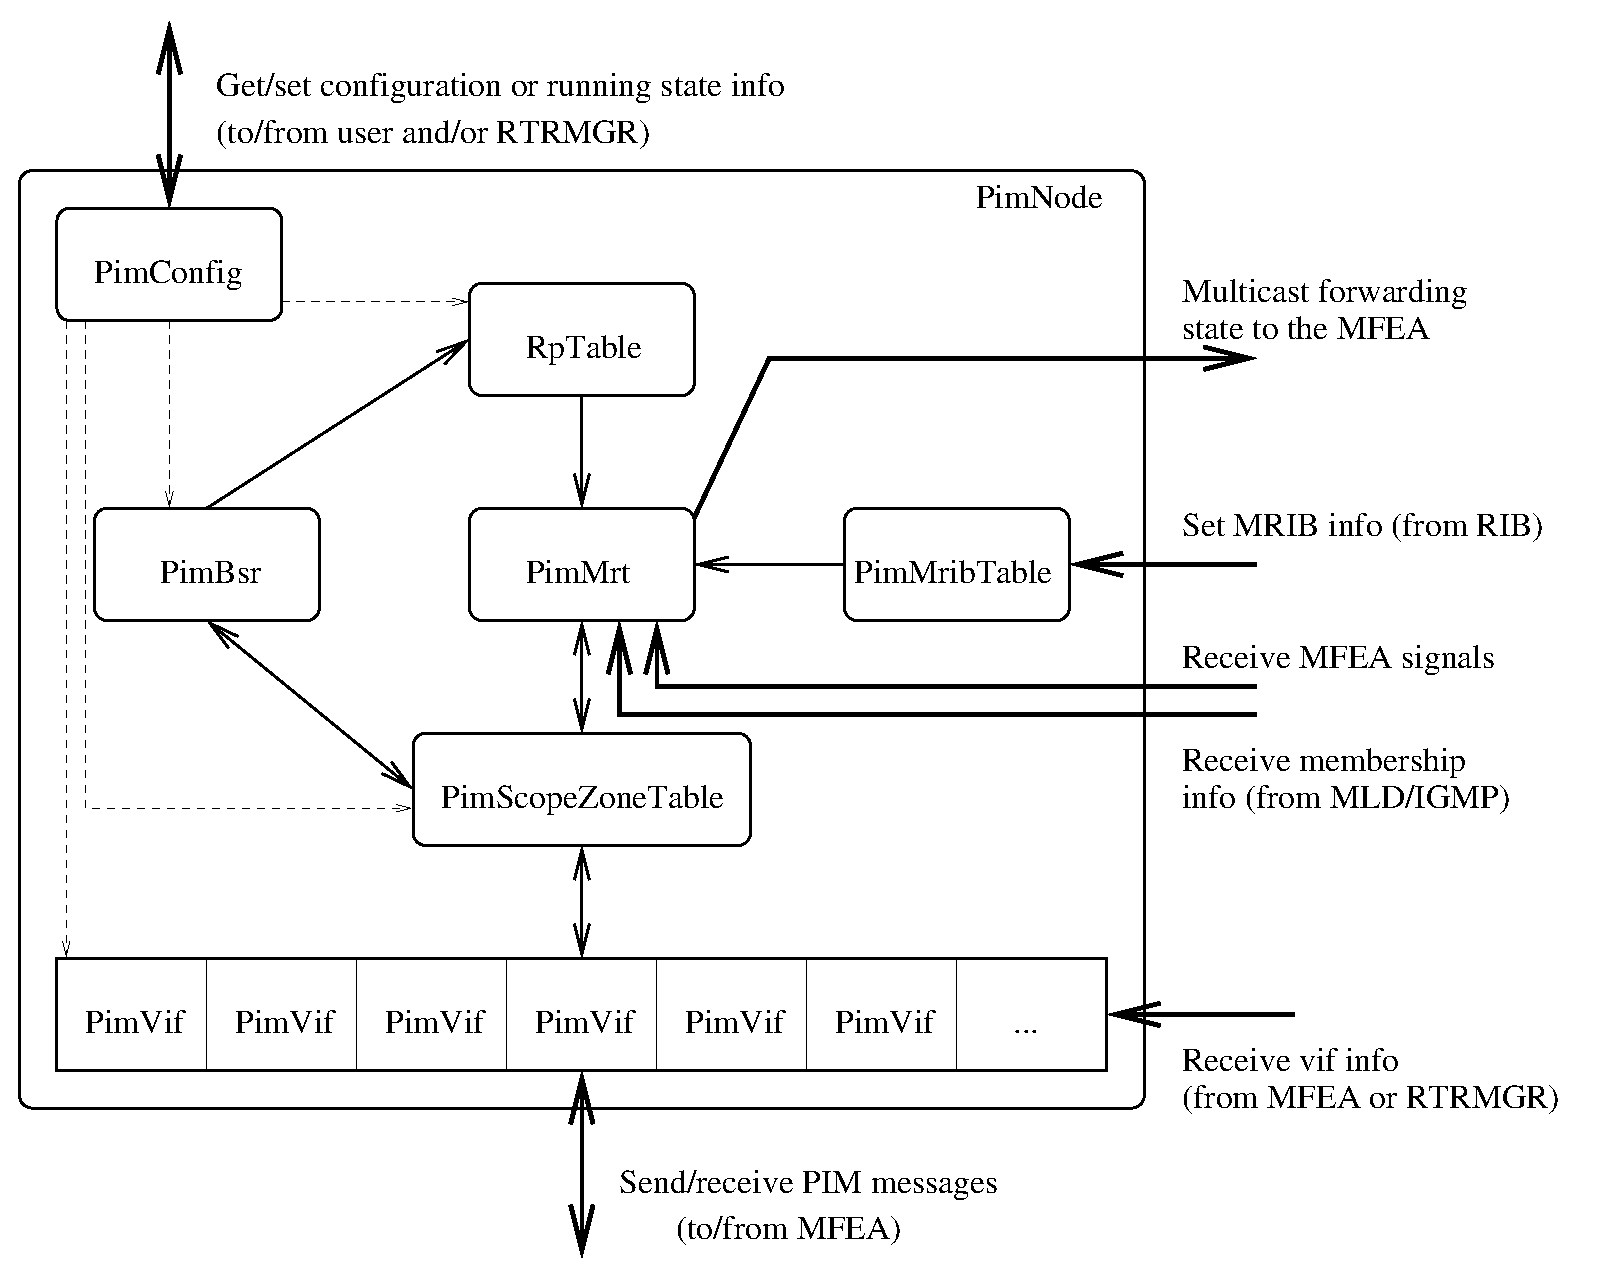
\includegraphics[width=6.0in]{figs/pim_design_overview}
    \caption{PIM-SM design overview}
    \label{fig:pim_design_overview}
  \end{center}
\end{figure}

Figure~\ref{fig:pim_design_overview} provides a general overview of the
PIM-SM components. For each component there is a C++ class with exactly
the same name. The main components are briefly described below:

\begin{itemize}

  \item {\bf PimNode:} a representation of a single PIM-SM routing unit
  (\eg a virtual PIM-SM router).
  Typically, there would be a single PimNode per PIM-SM router.

  \item {\bf PimVif:} PIM-specific virtual (network) interface that is used for
  sending and receiving PIM control packets.

  \item {\bf PimScopeZoneTable:} the table that contains information about
  scoped zones.

  \item {\bf PimMrt:} PIM-specific multicast routing table.

  \item {\bf PimBsr:} the PIM-Bootstrap mechanism unit.

  \item {\bf RpTable:} the table with the PIM-SM RP information.

  \item {\bf PimMribTable:} the table with the MRIB information.

  \item {\bf PimConfig:} contains PIM-specific configuration.

\end{itemize}

Those components are described in details in
Section~\ref{sec:components_description}.
For information about the interaction between the PIM-SM and other modules
see \cite{xorp:multicast_arch}.


%%%%%%%%%%%%%%%%%%%%%%%%%%%%%%%%%%%%%%%%%%%%%%%%%%%%%%%%%%%%%%%%%%%%%%%
\section{Components Description}
\label{sec:components_description}


%%%%%%%%%%%%%%%%%%%%%%%%%%%%%%%%%%%%%%%%%%%
\subsection{PimNode Description}

PimNode is a representation of a single PIM-SM routing unit (\eg a
virtual PIM-SM router).
Typically, there would be a single PimNode per PIM-SM router.
However, in some cases a PIM-SM router may have more than one
routing unit. For example, it could have one PimNode for IPv4, and
another one for IPv6 multicast routing. Further, if we want to
run PIM-SM in a simulation environment, each PIM-SM router within that
simulation will be represented by a single PimNode.

From a developer's point of view, PimNode contains all the state related to
the PIM-SM routing unit, and exports the front-end interface to interact with
that unit.
For example, PimNode contains the methods to
start/stop or configure PIM-SM, or to send/receive PIM control packets
to/from the routing unit. Those methods are described in the following files:

\begin{itemize}
  \item \verb=pim/pim_node.hh=
  \item \verb=libproto/proto_node.hh=
  \item \verb=libproto/proto_unit.hh=
\end{itemize}

PimNode itself does not implement the mechanisms to communicate with
other routing units (\eg to send or receive control packets to/from the
network), or to perform other PIM-independent operations such as
installing multicast forwarding entries in the multicast forwarding
engine. Those mechanisms are outside the scope of PimNode, and must be
implemented separately.

PimNode contains several pure virtual methods (\eg
\verb=join_multicast_group()= is used to join a multicast group on
an interface) that must be implemented by a class that inherits PimNode.
For example, XrlPimNode is a class that uses PimNode as a base class;
XrlPimNode uses XRL-based communication mechanisms between PimNode
and other XORP components such as the MFEA and MLD/IGMP modules.

By default, PimNode is disabled; therefore, on startup it must be enabled
explicitly.

%%%%%%%%%%%%%%%%%%%%%%%%%%%%%%%%%%%%%%%%%%%
\subsection{PimVif Description}

PimVif is a PIM-specific virtual (network) interface that is used for sending
and receiving PIM control packets. It includes the methods for processing and
composing PIM control messages, as well as various state per interface
(\eg the information about PIM-SM neighbors).

Typically, there would be one PimVif per network interface such as
physical interface, tunnel, or the loopback
interface. In addition, there would be one special PimVif virtual
interface: the PIM Register virtual interface that is used for sending
and receiving PIM Register messages. Not all virtual interfaces are
used by PIM; for example, all interfaces that are not multicast
capable, and the loopback interface are ignored for multicast
routing.

Typically, from developer's point of view, all interaction with PimVif
would be through PimNode~\footnote{For simplicity, currently (June 2003)
there are few occasions when XrlPimNode uses direct access to PimNode.}.

The public interface for PimVif contains the methods to manipulate a
virtual (network) interface. Those methods are to start/stop/enable/disable a
virtual interface, and to configure it. The methods are described in
the following files:

\begin{itemize}
  \item \verb=pim/pim_vif.hh=
  \item \verb=libxorp/vif.hh=
  \item \verb=libproto/proto_unit.hh=
\end{itemize}

PimVif contains state such as PIM Hello related information. Also, all
the PIM-specific methods for parsing or constructing PIM control
messages when a PIM packet is received or sent are implemented as
methods in PimVif. The parsing or construction of each message type is
implemented in a separate file with a name prefix of \verb=pim_proto=.
For example, \verb=pim_proto_cand_rp_adv.cc= implements sending and
receiving of PIM Candidate-RP-Advertisement messages. The handing of
other message types is implemented in similarly named files.

By default, each PimVif is disabled; therefore, on startup it must be
enabled explicitly. 


%%%%%%%%%%%%%%%%%%%%%%%%%%%%%%%%%%%%%%%%%%%
\subsection{PimScopeZoneTable Description}

PimScopeZoneTable is a table that contains information about scoped
zones. There is one such table per PimNode. This table is used to check
whether various control messages are allowed to be sent or accepted a
specific network interface~\footnote{Note that in the current implementation
(June 2003) the PimScopeZoneTable is used only for PIM
Bootstrap messages. In the future, the scope zone information would be
used for other control messages as well.}.

By default, PimScopeZoneTable is empty; \ie there are no scoping zone
restrictions.


%%%%%%%%%%%%%%%%%%%%%%%%%%%%%%%%%%%%%%%%%%%
\subsection{PimMrt Description}

PimMrt is the PIM-specific multicast routing table. It is the central
and most important component: its state is modified by the PIM control
messages, and the output of it is the multicast forwarding state
information that is installed in the multicast forwarding engine.

The multicast routing table is composed of four tables. Each table
contains PimMre entries (described in file \verb=pim/pim_mre.hh=):

\begin{itemize}

  \item (*,*,RP) multicast routing table. This table contains all
  (*,*,RP) multicast routing entries~\footnote{(*,*,RP) entry is an
  entry that matches all multicast groups that use one specific
  RP.}. For simplicity of implementation, this table contains an
  (*,*,RP) entry for each RP in the RpTable, even if no (*,*,RP) Join
  messages for that RP were received.  The iterator for this table
  returns the entries ordered by their RP address: the numerically
  smallest addresses first. Note that each PimMre entry in this table
  has the source address set to the RP address, and the group address
  set to zero (\ie \verb=IPvX::ZERO()=).

  \item (*,G) multicast routing table. This table contains all (*,G)
  multicast routing entries. Each entry in that table contains a pointer
  to the corresponding (*,*,RP) entry for that group, or NULL if the
  group has no RP yet. The iterator for this table returns the entries
  ordered by their group address: the numerically smallest addresses
  first. Note that each PimMre entry in this table has the source
  address set to zero (\ie \verb=IPvX::ZERO()=).

  \item (S,G) multicast routing table. This table contains all (S,G)
  multicast routing entries. Each entry in that table contains a pointer
  to the corresponding (*,G) entry for that group, or NULL if there is
  no (*,G) entry. It also contains a pointer to the corresponding
  (S,G,rpt) entry if such entry exists (seen below). There are two iterators
  for this table: an iterator for the entries ordered by the numerically
  smallest source address first, and an iterator for the entries ordered
  by the numerically smallest group address first.

  \item (S,G,rpt) multicast routing table. This table contains all
  (S,G,rpt) multicast routing entries. Each entry in that table contains
  a pointer to the corresponding (*,G) entry for that group, or NULL if
  there is no (*,G) entry. It also contains a pointer to the
  corresponding (S,G) entry if such entry exists. There are two
  iterators for this table: an iterator for the entries ordered by the
  numerically smallest source address first, and an iterator for the
  entries ordered by the numerically smallest group address first.

\end{itemize}

For simplicity of implementation, currently (June 2003) PimMrt
contains one more table: PimMrtMfc PIM-specific table with Multicast
Forwarding Cache (PimMfc) entries (in the future, this table may be
moved out of PimMrt to PimNode). This table contains all
entries that have been installed in the multicast forwarding table in
the multicast forwarding engine. Currently (June 2003), those
entries are source-group-specific, and are installed ``on-demand'' (\ie
only if there is an active source for some multicast group). In the future,
group-specific entries may be supported as well (assuming that that
multicast forwarding engine supports (*,G) multicast forwarding
entries).

In addition to the above tables, PimMrt contains a mechanism for
tracking dependencies among the PimMre and PimMfc entries, as well as
the PimMre and PimMfc dependencies on external state such as the RP set
or the MRIB information. For example, if the MRIB for a specific network
prefix changes, then all PimMre and PimMfc entries that depend on that
network prefix must be updated accordingly. A single change may trigger
a number of operations that must be performed on a number of entries,
therefore we need to carefully track the state dependency. Below is a
summary of some of the events that may trigger actions to process
entries in PimMrt:

\begin{itemize}

  \item RP-Set change: \eg if there is any change to the RP-Set that
  affects the group-to-RP mapping.

  \item MRIB change: any change in the underlying unicast routing that
  affects the Reverse-Path Forwarding information toward an RP or a
  source.

  \item Next-Hop PIM neighbor change: any change to the set of PIM
  neighbors that may affect the Next-Hop PIM Router toward a destination.

  \item Reception of a PIM Join/Prune message.

  \item Reception of a PIM Assert message.

  \item Add/deletion of a local multicast member.

  \item Change in the Designated Router on an interface.

  \item Change in the IP address or IP subnet on an interface.

  \item Start or stop a virtual interface.

  \item Addition or deletion of a PimMre entry.

\end{itemize}

A complete list of all input events that may trigger actions is in file
\verb=pim/pim_mre_track_state.hh= (see the
\verb=input_state_t INPUT_STATE_*= events).

In some cases, keeping track of the entries that need to be processed
for a given input event is relatively simple. For example, if the MRIB
for a network prefix changes, processing all (S,G) PimMre entries that
might be affected can be done by using the source-first iterator for the
(S,G) multicast routing table, and then iterating over all (S,G) PimMre
entries whose source address matches that network prefix. However, in
other cases we cannot use those table iterators. For example, if an RP is
deleted, we need to process all corresponding (*,G) entries that match
to that RP, and to reassign them to a new RP. In that case, to keep track
of the dependencies between the RP and the (*,G) entries, each RP entry
in the RpTable contains a list of PimMre entries that match to that
RP. Similarly, each PimNbr entry (an entry that contains information
about a PIM neighbor) contains a list of all PimMre entries that use
that PIM neighbor as the Next-Hop Router toward the RP or the source.

The dependency tracking mechanism needs to solve another problem: for
each input event, find all the operations and their ordering that need
to be performed on some of the PimMre and PimMfc entries.  The solution
chosen to solve this problem is to enumerate all possible input events
and output operations, and to compute in advance a table. Lookup to this
table for a given input event returns a list of the ordered output
operations that need to be performed for that event.

If there are just few input events and output operations, it might be
possible to create such table manually. However, currently (June
2003) there are 52 input events and 75 output operations,
therefore it is not feasible to crate manually such table.
The solution is on startup to automatically compute this table based on
a set of rules about the various state dependencies as defined in the
PIM-SM spec. Those state dependencies are derived from the macros in the
PIM-SM protocol specification. For example, the specification document
contains macros like:

\begin{verbatim}
pim_include(S,G) =
    { all interfaces I such that:
      ( (I_am_DR( I ) AND lost_assert(S,G,I) == FALSE )
        OR AssertWinner(S,G,I) == me )
       AND  local_receiver_include(S,G,I) }
\end{verbatim}

Then, the corresponding state dependency rule in the implementation is:

\begin{verbatim}
void
PimMreTrackState::track_state_pim_include_sg(list<PimMreAction> action_list)
{
    track_state_i_am_dr(action_list);
    track_state_lost_assert_sg(action_list);
    track_state_assert_winner_sg(action_list);
    track_state_local_receiver_include_sg(action_list);
}
\end{verbatim}

In other words, if the value of \verb=lost_assert(S,G,I)= for example changes,
then the value of \verb=pim_include(S,G)= must be recomputed.
However, we may have some state dependency rules for
\verb=lost_assert(S,G,I)= itself, hence if we combine all state
dependency rules, we can represent the dependencies with a collection
of uni-directional graphs. Then, to create the list of actions for each
input entry, we need to consider all paths from the graph node for
that input entry to all reachable output actions.
The uni-directional graphs creation and the extraction of the lists of
actions for each input entry is performed once on startup. The result
lists are saved internally inside PimMrt, and used during processing of
input actions.

Finally, the last major problem that the dependency tracking mechanism
needs to solve is how to process a large number of entries triggered by
a single event without stopping processing of other components in the
router (\eg receiving PIM control packets, or responding to a command
sent by the CLI). This problem requires attention
because the implementation is single-threaded, therefore if processing a
single event takes too long, the rest of the pending events may
be processed too late (\eg if the periodic sending of PIM Hello messages
is delayed for too long, the PIM neighbors may timeout this
router). The solution of this problem is to voluntarily suspend
the processing if it is taking too long, then save the necessary state
to continue the processing sometime later, and finally return control to
the control loop which handles all events. Typically, the processing of
some event may take too
long if there is a large number of PimMre or PimMrt entries that
need to be processed (for example, thousands of (*,G) entries if the RP
for those entries changes). In that case, we use ``time-slices'' to
compute how long has taken the processing so far.
In the above example, we check the processing time after we process each
(*,G) entry: if the elapsed time is above a threshold (default to 100ms
as of June 2003), we save the appropriate state to continue the
processing later (\eg in the above example we save the address of the
next multicast group to process).

All dependency tracking processing and time-slicing uses PimMreTask
entries to keep the appropriate state. There is a single list of
PimMreTask entries per PimNode, and the list is FIFO: new tasks are
added to the end of the lists, and the task at the front of the list is
processed until it is completed (\eg within one or several time-slices).

%%%%%%%%%%%%%%%%%%%%%%%%%%%%%%%%%%%%%%%%%%%
\subsection{PimBsr Description}

PimBsr is the PIM-Bootstrap mechanism unit. It implements the Bootstrap
mechanism as described in \cite{PIM-SM-BOOTSTRAP}. There is one PimBsr
unit per PimNode. The main purpose of the PimBsr is to run the Bootstrap
mechanism, and to update accordingly the RpTable with the current RP-Set.

The data contained in PimBsr is organized as described below.
PimBsr keeps three lists of BsrZone entries: one list for the active BSR
zones, a second list that contains information about expiring Candidate-RPs for
group prefixes that the lastest Bootstrap message did not contain information
about, and a third list for the locally configured Cand-BSR zones and/or
Cand-RP information. On startup, the active and expire BSR zone lists are
empty. If the node is configured as a Candidate-BSR and/or a Candidate-RP,
this information will be added to the third list; otherwise that list is 
also empty.

Each scope zone is identified by a scope zone ID, and a flag.
The flag, if true, indicates that this is scoped zone, otherwise the
zone is non-scoped. The scope zone ID is the network prefix address that
corresponds to that zone. By definition, scoped zones cannot overlap,
therefore it is not permitted to configure the PimBsr with overlapping
scoped zones and/or to accept Bootstrap messages with scoped zones that
overlap. If the zone is non-scoped, then the scope zone ID is set to the
multicast base prefix address (\ie 224.0.0.0/4 for IPv4 or FF00::/8 for
IPv6).

Each BsrZone contains information about the current BSR for that zone,
and a list of BsrGroupPrefix entries for that zone. Each BsrGroupPrefix
corresponds to a multicast group prefix within that zone that has
Candidate-RPs, and contains the list of BsrRp entries for each
Candidate-RP for that prefix.

All information from the Bootstrap and Candidate-RP messages is kept in
the above data structures. Further, those structures are used to keep
various timers such as to timeout Candidate RPs or to timeout the current BSR.
If the RP-Set is changed after receiving a Bootstrap message or after a
timeout of an Candidate-RP, then the RpTable is updated accordingly.


%%%%%%%%%%%%%%%%%%%%%%%%%%%%%%%%%%%%%%%%%%%
\subsection{RpTable Description}

RpTable is the table that contains the current RP-Set. There is one
table per PimNode. This table is updated by PimBsr if the RP-Set is
propagated through the Bootstrap mechanism, or by PimConfig if the
RP-Set is configured manually.

RpTable contains a list of all RPs with one PimRp entry per RP per
multicast group prefix. To compute the RP for a given group,
we just scan the whole list to find the RP.
Typically, the list of RPs would be relatively short, therefore for
simplicity we scan the whole list. If the overhead becomes too large,
then the scan can be optimized by grouping the Candidate-RPs
for each group prefix, and by considering only the Candidate-RPs with
the highest priority.

If the RP-Set is modified, then all affected PimMre and PimMfc entries
must be updated accordingly. For this reason, each PimRp entry contains
lists of the PimMre and PimMfc entries that map to that RP. If the RP
is removed, then each of the entries on those lists is re-mapped to the
new RP for its group.
This is achieved by scheduling a PimMreTask by the PimMrt,
that performs the appropriate dependency actions for each entry.

The RpTable may contain one special PimRp entry with an RP address of
all-zeroes (\ie \verb=IPvX::ZERO()=). This entry is used to keep the
lists of all PimMre and
PimMfc entries that have no RP yet. If a new RP is added to the RpTable,
then all entries that have no RP yet are processed to find if some
of them may map to this new RP. Those who do map to the new RP are moved to
the appropriate list for that RP.


%%%%%%%%%%%%%%%%%%%%%%%%%%%%%%%%%%%%%%%%%%%
\subsection{PimMribTable Description}

PimMribTable is the table with the MRIB information. The MRIB is used
to compute the Reverse-Path Forwarding information toward the RPs
(needed by the (*,*,RP), (*,G) and (S,G,rpt) state), and toward
each active multicast sender (needed by the (S,G) state). This
information contains the next-hop router address and the interface
toward that router, the routing metric and the metric preference:

{\small
\begin{verbatim}
// Reverse-Path Forwarding information (MRIB payload entry)
class Mrib {
    ...
    IPvXNet     _dest_prefix;          // The destination prefix address
    IPvX        _next_hop_router_addr; // The address of the next-hop router
    uint16_t    _next_hop_vif_index;   // The vif index to the next-hop router
    uint32_t    _metric_preference;    // The metric preference to the
                                       // destination
    uint32_t    _metric;               // The metric to the destination
};
\end{verbatim}
} % \small


The MRIB information is obtained from the RIB
module~\footnote{Currently (June 2003), the information is
received from the MFEA instead.}; if the RIB changes, the
PimMribTable is updated as well. Examples when the MRIB information
may change are: the unicast routing changes the next-hop router address
toward a destination, local configuration changes some of the routing
preference metrics, or local interface configuration changes the virtual
interface and/or the next-hop router toward a destination.

An update to the PimMribTable may affect a number of PimMre and PimMfc
entries in the PimMrt table. The update of the affected entries is
handled by the dependency-tracking and time-slice processing mechanism
implemented by the PimMrt table. Note that we do not need to link all
PimMre and PimMfc entries into lists of entries that depend on a
particular entry in the PimMribTable. The reason is because the
dependency is implied by the network prefix address covered by an entry
in the PimMribTable, that overlaps the RP or source address of a given
PimMre or PimMfc entry.

%%%%%%%%%%%%%%%%%%%%%%
\subsubsection{MRIB Changes Update}

In general, there are two mechanisms to inform the PIM-SM module about
MRIB changes:

\begin{itemize}
  \item \emph{Filtering at the PIM-SM module:}
  Whenever there are any changes about the MRIB information kept inside
  the RIB module, the RIB module informs the PIM-SM module
  about the changes. Then the PIM-SM module processes those changes to
  find whether they would affect in any way the current multicast
  routing.

  \item \emph{Filtering at the RIB module:}
  The PIM-SM module ``registers'' in advance with the RIB module about
  the particular destination addresses/prefixes it is interested at, and
  only if the MRIB information about any of those registered destinations
  is changed, the RIB module informs the PIM-SM module about the change.

\end{itemize}

The basic difference between the above two methods is where we move the
complexity about the MRIB changes: at the RIB side, or the PIM-SM side.
Some other differences are:

\begin{itemize}
  
  \item If we perform filtering at the PIM-SM module, and if the unicast
  routing is changing quite rapidly, and if most of those changes do not
  affect the PIM-SM module, this will add unnecessary overhead to the
  communication from the RIB to the PIM-SM module.
  
  \item If we perform filtering at the RIB module, and if there is a
  large number of destinations the PIM-SM module needs to be informed
  about, registering all of those destinations at the RIB may introduce
  an ``explosion'' of communication from the RIB to the PIM-SM module
  in case when there is a change in the routing information about a
  large number of destinations.
  
  \item If we perform filtering at the PIM-SM module, the implementation
  may require the PIM-SM to keep a local (simplified) copy of all the
  RIB information, therefore it may increase notably the memory usage.
  This copy however can be used to perform the proper comparison and
  modification whenever MRIB update is received from the RIB module.
  
\end{itemize}

It may be possible to use some hybrid methods of propagating the MRIB
changes from the RIB module to the PIM-SM module, but based on the
above comparison it seems that \emph{filtering at the PIM-SM module} is
the simpler and more appropriate solution. Therefore, the RIB module
needs to inform the PIM-SM module whenever the MRIB information for any
destination prefix is changed.  The simplest solution for the RIB
module would be whenever any entry is changed, the RIB module would
``dump'' all RPF entries. This however may increase the communication
overhead, and may complicate additionally the PIM-SM module. A better
solution would be if the RIB modules sends only atomic updates of the
RPF information to the PIM-SM module. For example, a single message
would contain all affected entries: \eg a list of \emph{MRIB\_ADD} and
\emph{MRIB\_DELETE} commands, and the particular ordering of those
entries would specify also the order the PIM-SM module should apply
them.

Note that as we mentioned earlier, currently (June 2003), the MRIB
information is received from the MFEA, which reads directly the unicast
forwarding table from the (UNIX) kernel, and PIM-SM keeps a local copy
of the whole table. The MFEA periodically reads (\eg every 10 seconds)
the unicast forwarding table, and if there is any change, it sends the
changes to all interested modules (that includes the PIM-SM module).
Similarly, the MFEA informs PIM-SM about any virtual interfaces
information changes (\eg an address has been added or
deleted)~\footnote{Strictly speaking, the VIF (Virtual InterFace)
abstraction is based on 
information that can be obtained directly from the kernel. However, the
VIF information is also related with the RIB information as well,
therefore for consistency reason, probably it is better if any VIF
information changes is propagated via the RIB module to the PIM-SM
module, especially because any change in the VIF information may affect
the unicast routing as well. This is an open issue, therefore in the
future the current behavior may be changed.}.

%%%%%%%%%%%%%%%%%%%%%%%%%%%%%%%%%%%%%%%%%%%
\subsection{PimConfig Description}

PimConfig handles the PIM-specific configuration~\footnote{Currently
(June 2003), PimConfig is not implemented; rather, all state is
kept inside PimNode instead.}. This configuration is used to configure the
following units:

\begin{itemize}

  \item PimVif: protocol version, Hello-related options and timer
  values, etc.

  \item PimScopeZone table: add and delete information about scoped zones.

  \item PimBsr: configure the local routing unit as a Candidate-BSR or a
  Candidate-RP.

  \item RpTable: add static RPs to the RP-Set.

\end{itemize}


%%%%%%%%%%%%%%%%%%%%%%%%%%%%%%%%%%%%%%%%%%%%%%%%%%%%%%%%%%%%%%%%%%%%%%%
%     APPENDIX
%%%%%%%%%%%%%%%%%%%%%%%%%%%%%%%%%%%%%%%%%%%%%%%%%%%%%%%%%%%%%%%%%%%%%%%
\appendix
\section{Modification History}

\begin{itemize}

  \item December 11, 2002: Version 0.1 completed.

  \item March 10, 2003: Updated to match XORP version 0.2 release code;
  cleanup.

  \item June 9, 2003: Bump-up the version to 0.3, and the date.

\end{itemize}


%%%%%%%%%%%%%%%%%%%%%%%%%%%%%%%%%%%%%%%%%%%%%%%%%%%%%%%%%%%%%%%%%%%%%%%
%     BIBLIOGRAPHY
%%%%%%%%%%%%%%%%%%%%%%%%%%%%%%%%%%%%%%%%%%%%%%%%%%%%%%%%%%%%%%%%%%%%%%%
\bibliography{../tex/xorp}
\bibliographystyle{plain}

%%%%%%%%%%%%%%%%%%%%%%%%%%%%%%%%%%%%%%%%%%%%%%%%%%%%%%%%%%%%%%%%%%%%%%%
\end{document}
